\documentclass[tikz,border=8pt]{standalone}
\usepackage{amsmath,amssymb}
\usetikzlibrary{arrows.meta,automata,positioning,quotes}
\begin{document}
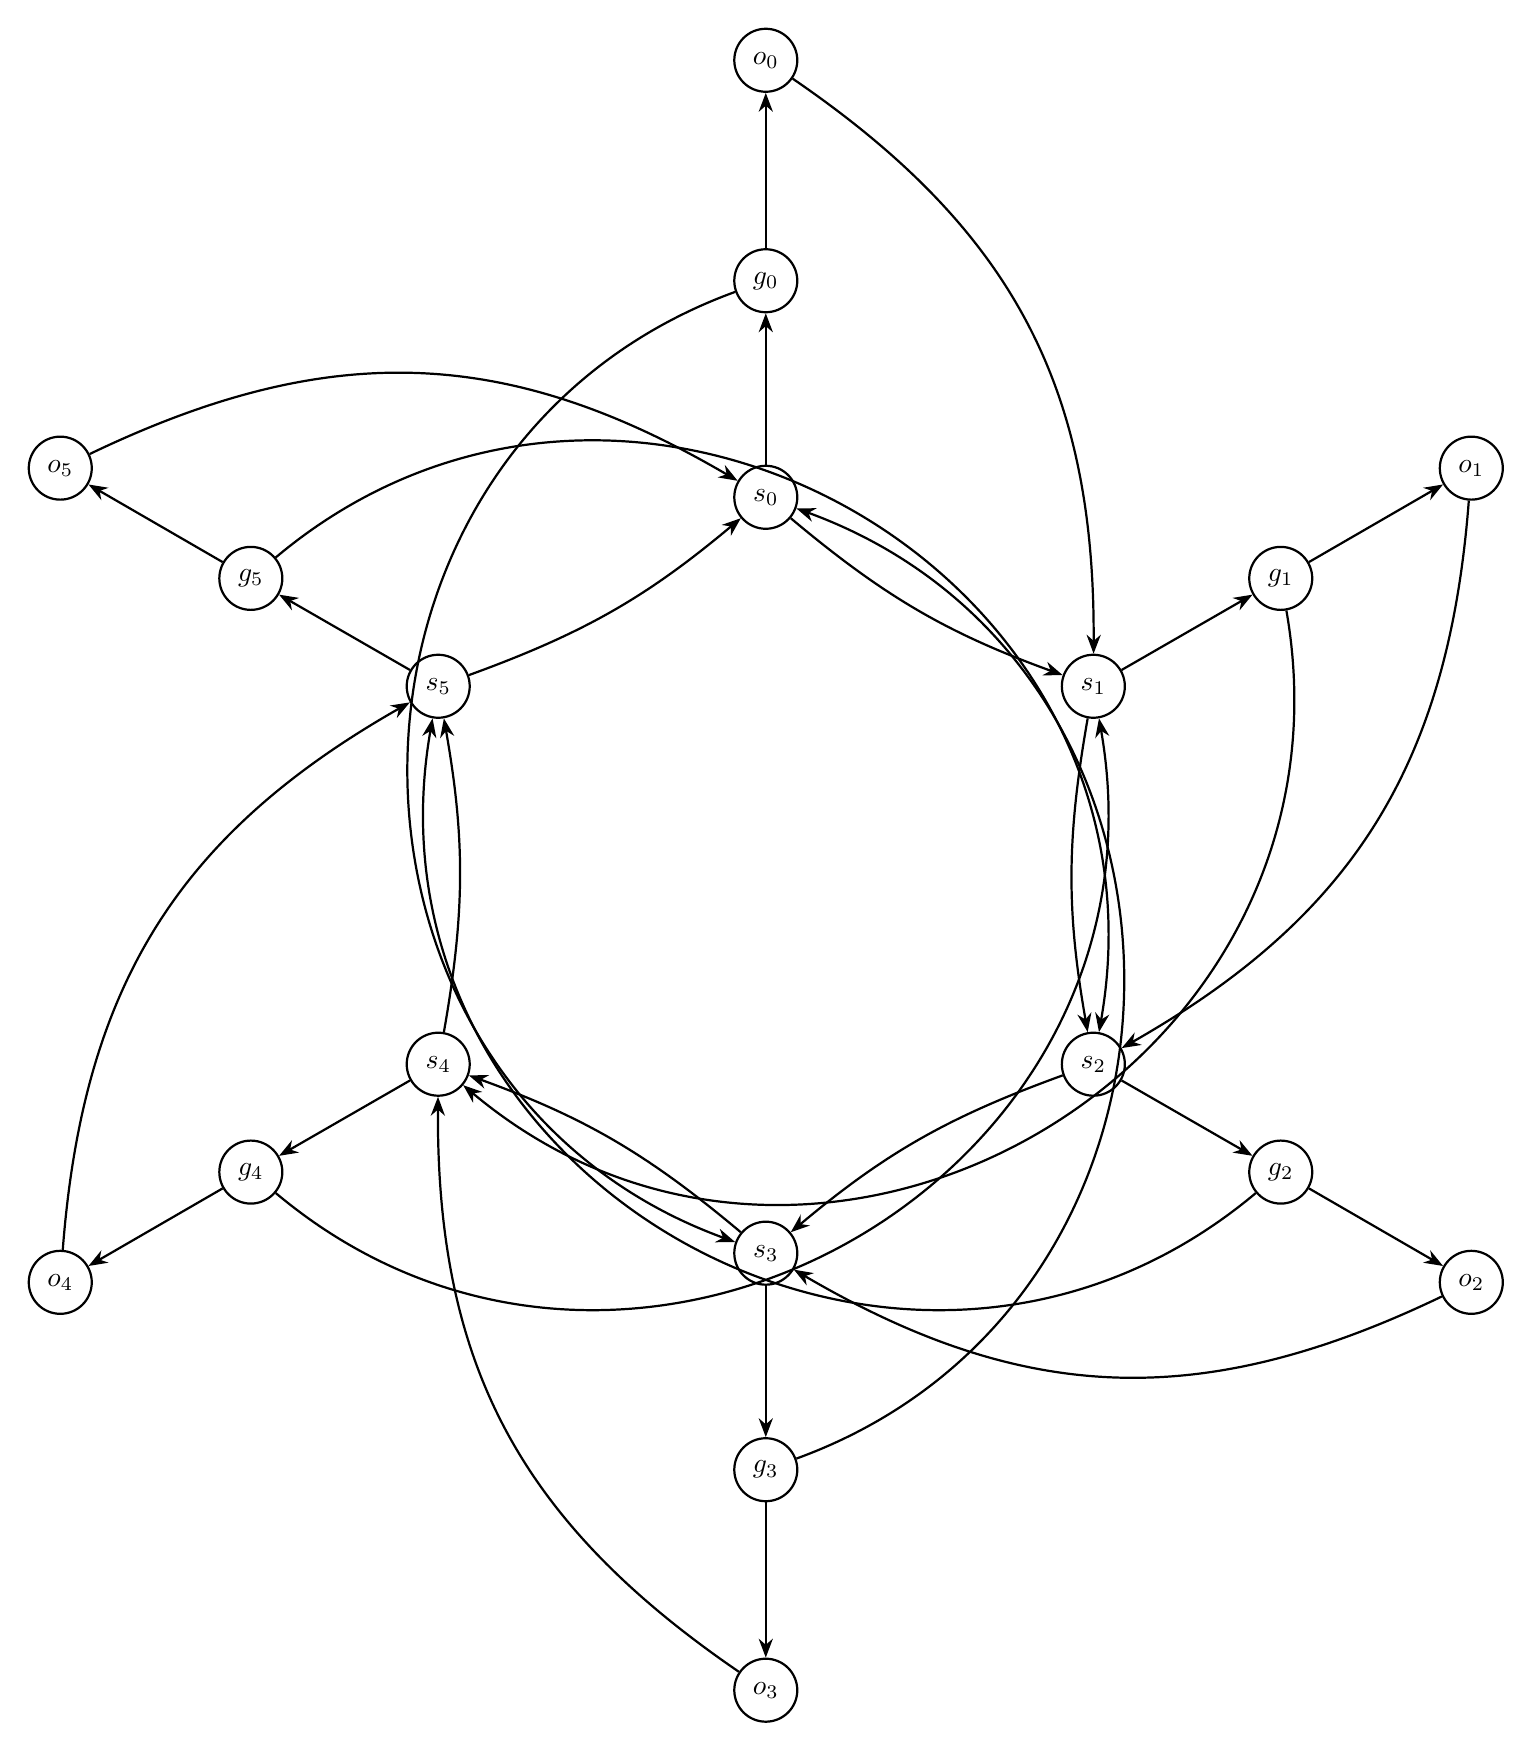
\begin{tikzpicture}[x=1cm,y=1cm]
\tikzset{
  graphnode/.style={circle,draw,thick,minimum size=8mm,inner sep=1pt,font=\sffamily},
  directed/.style={-{Stealth[length=2.4mm]},thick},
  undirected/.style={thick}
}
\node[graphnode] (n_s0) at (0.00,4.80) {$s_0$};
\node[graphnode] (n_s1) at (4.16,2.40) {$s_1$};
\node[graphnode] (n_s2) at (4.16,-2.40) {$s_2$};
\node[graphnode] (n_s3) at (0.00,-4.80) {$s_3$};
\node[graphnode] (n_s4) at (-4.16,-2.40) {$s_4$};
\node[graphnode] (n_s5) at (-4.16,2.40) {$s_5$};
\node[graphnode] (n_g0) at (0.00,7.55) {$g_0$};
\node[graphnode] (n_g1) at (6.54,3.77) {$g_1$};
\node[graphnode] (n_g2) at (6.54,-3.77) {$g_2$};
\node[graphnode] (n_g3) at (0.00,-7.55) {$g_3$};
\node[graphnode] (n_g4) at (-6.54,-3.77) {$g_4$};
\node[graphnode] (n_g5) at (-6.54,3.77) {$g_5$};
\node[graphnode] (n_o0) at (0.00,10.35) {$o_0$};
\node[graphnode] (n_o1) at (8.96,5.17) {$o_1$};
\node[graphnode] (n_o2) at (8.96,-5.17) {$o_2$};
\node[graphnode] (n_o3) at (0.00,-10.35) {$o_3$};
\node[graphnode] (n_o4) at (-8.96,-5.17) {$o_4$};
\node[graphnode] (n_o5) at (-8.96,5.17) {$o_5$};
\draw[directed] (n_s0) to[bend right=10,looseness=1] (n_s1);
\draw[directed] (n_s1) to[bend right=10,looseness=1] (n_s2);
\draw[directed] (n_s2) to[bend right=10,looseness=1] (n_s3);
\draw[directed] (n_s3) to[bend right=10,looseness=1] (n_s4);
\draw[directed] (n_s4) to[bend right=10,looseness=1] (n_s5);
\draw[directed] (n_s5) to[bend right=10,looseness=1] (n_s0);
\draw[directed] (n_s0) -- (n_g0);
\draw[directed] (n_g0) -- (n_o0);
\draw[directed] (n_o0) to[bend left=28,looseness=1.05] (n_s1);
\draw[directed] (n_s1) -- (n_g1);
\draw[directed] (n_g1) -- (n_o1);
\draw[directed] (n_o1) to[bend left=28,looseness=1.05] (n_s2);
\draw[directed] (n_s2) -- (n_g2);
\draw[directed] (n_g2) -- (n_o2);
\draw[directed] (n_o2) to[bend left=28,looseness=1.05] (n_s3);
\draw[directed] (n_s3) -- (n_g3);
\draw[directed] (n_g3) -- (n_o3);
\draw[directed] (n_o3) to[bend left=28,looseness=1.05] (n_s4);
\draw[directed] (n_s4) -- (n_g4);
\draw[directed] (n_g4) -- (n_o4);
\draw[directed] (n_o4) to[bend left=28,looseness=1.05] (n_s5);
\draw[directed] (n_s5) -- (n_g5);
\draw[directed] (n_g5) -- (n_o5);
\draw[directed] (n_o5) to[bend left=28,looseness=1.05] (n_s0);
\draw[directed] (n_g0) to[bend right=70,looseness=1.25] (n_s3);
\draw[directed] (n_g1) to[bend left=70,looseness=1.25] (n_s4);
\draw[directed] (n_g2) to[bend left=70,looseness=1.25] (n_s5);
\draw[directed] (n_g3) to[bend right=70,looseness=1.25] (n_s0);
\draw[directed] (n_g4) to[bend right=70,looseness=1.25] (n_s1);
\draw[directed] (n_g5) to[bend left=70,looseness=1.25] (n_s2);
\end{tikzpicture}
\end{document}
